%!TEX root = THinstituteReport_1.tex


%%%%%%%%%%%%%%%%%%%%%%%%%%%%%%%%%%%%%%%%
\section{Monte Carlo studies}
\subsection{ToyModels}
%%%%%%%%%%%%%%%%%%%%%%%%%%%%%%%%%%%%%%%%

In order to study the impact of a high $k_{T}$ particle in the declustering process, we have performed a simple toy model where we generate Pythia jets to which we add an additional hard track prior to reclustering. The added hard track follows a $1/k_{T}^{4}$ and a $1/\omega$ distribution. 

Fig \ref{fig:toymodeltracks} shows the x and y projections of the Lund plot for the injected tracks and for the difference plot (Pythia jets with injected track relative to Pythia jets). In the left plot, that corresponds to CA declustering, we see that when we inject the tracks, there is an excess of splittings at large angle that does not overlap with the injected track distribution. We also see that the "contaminated" jets show an enhancement of low log(z $\theta$) relative to default jets that does not match the input injected track distribution. 
In the case of $k_{T}$ decustering (middle plot) we see that the angular distribution of the excess of splittings in the "contaminated" jets matches better that of the injected tracks. 
In the case of anti-$k_{T}$ (right plots) the excess of tracks in the contaminated jets appear at momentum scales that are lower than that of the injected tracks and the angular distribution appears shifted to higher values. 

This exercise was done to illustrate an idea that might seem trivial: if a particle is added to the jet, the splitting map is distorted in different regions of phase space depending on the declustering strategy. The distorsions in the splitting map seem to match better the regions were the extra particles were injected, in the case of $k_{T}$ declustering. 

\begin{figure}[h]
\centering
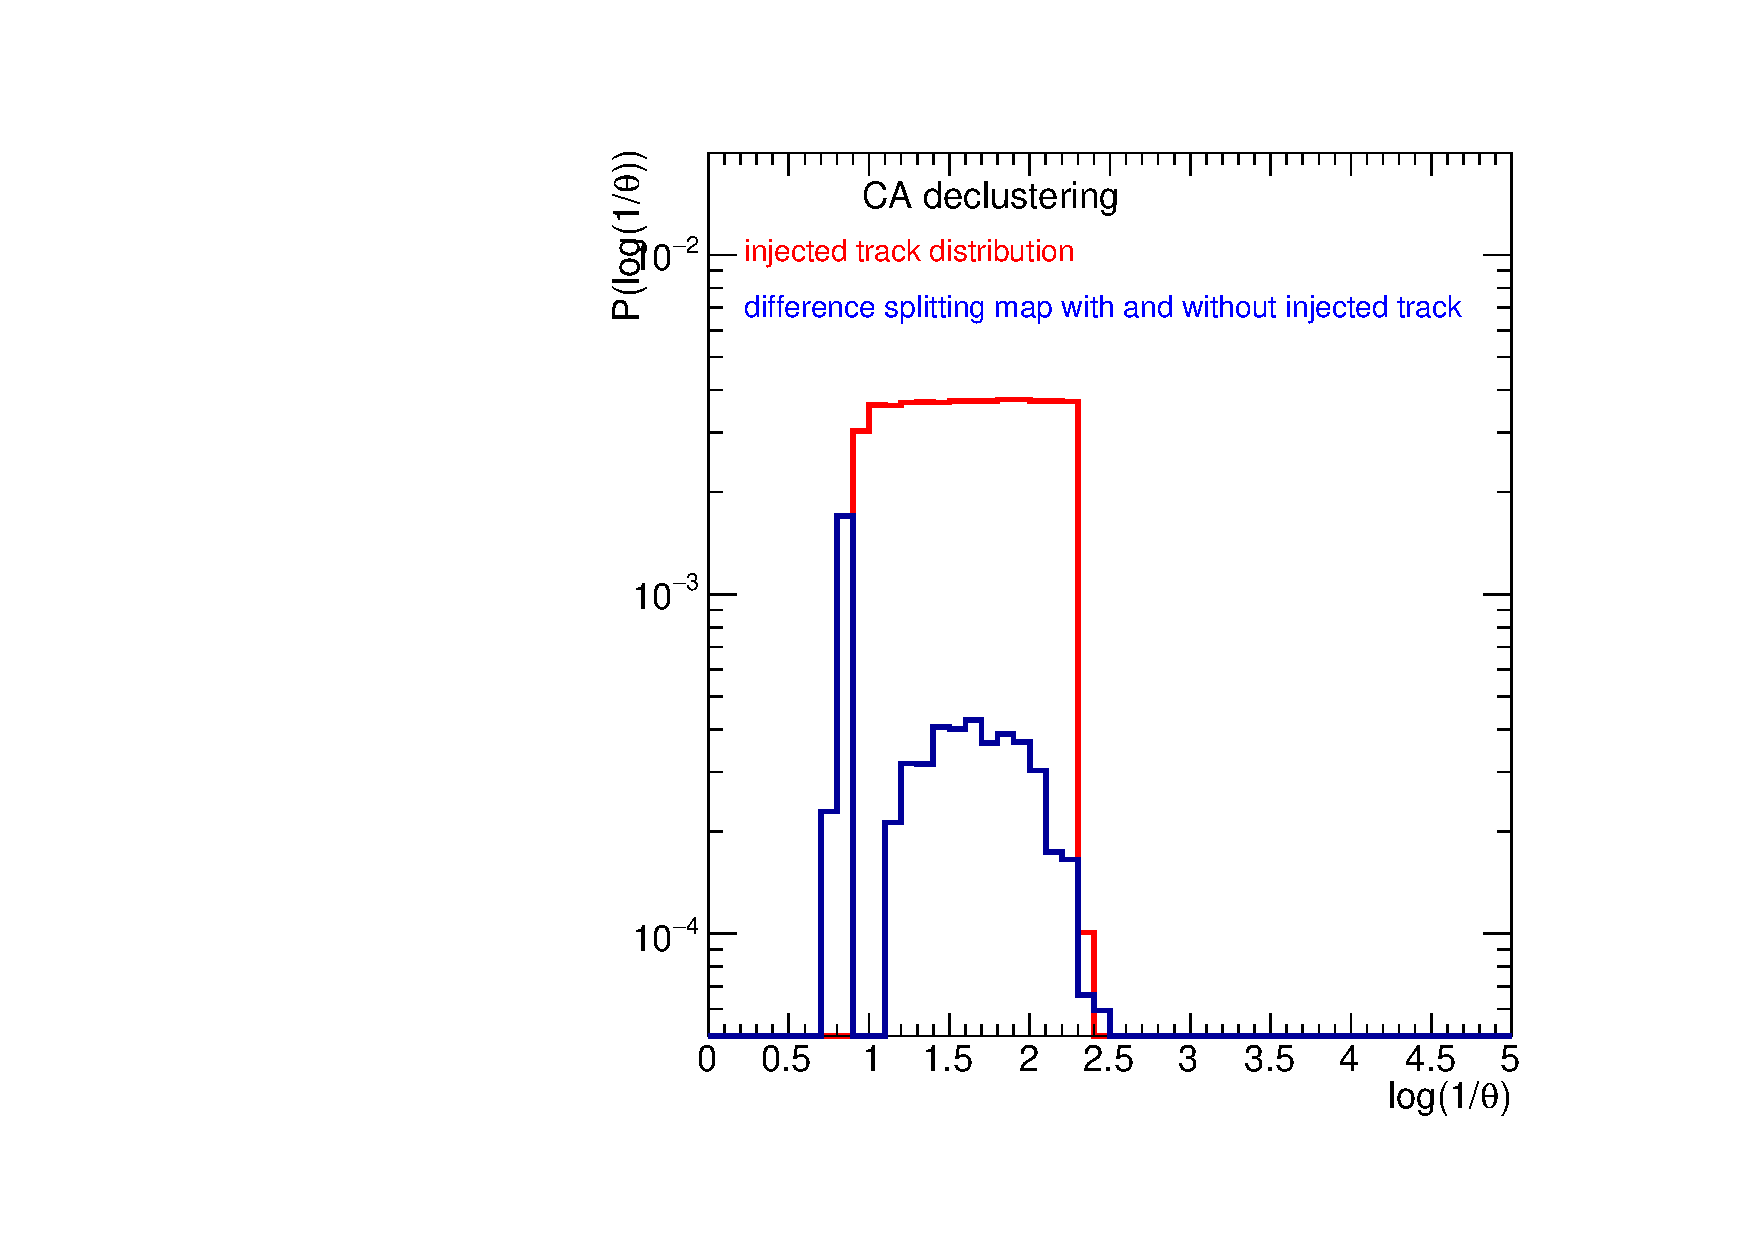
\includegraphics[width=0.3\textwidth]{figures/LundMC/projectxca}
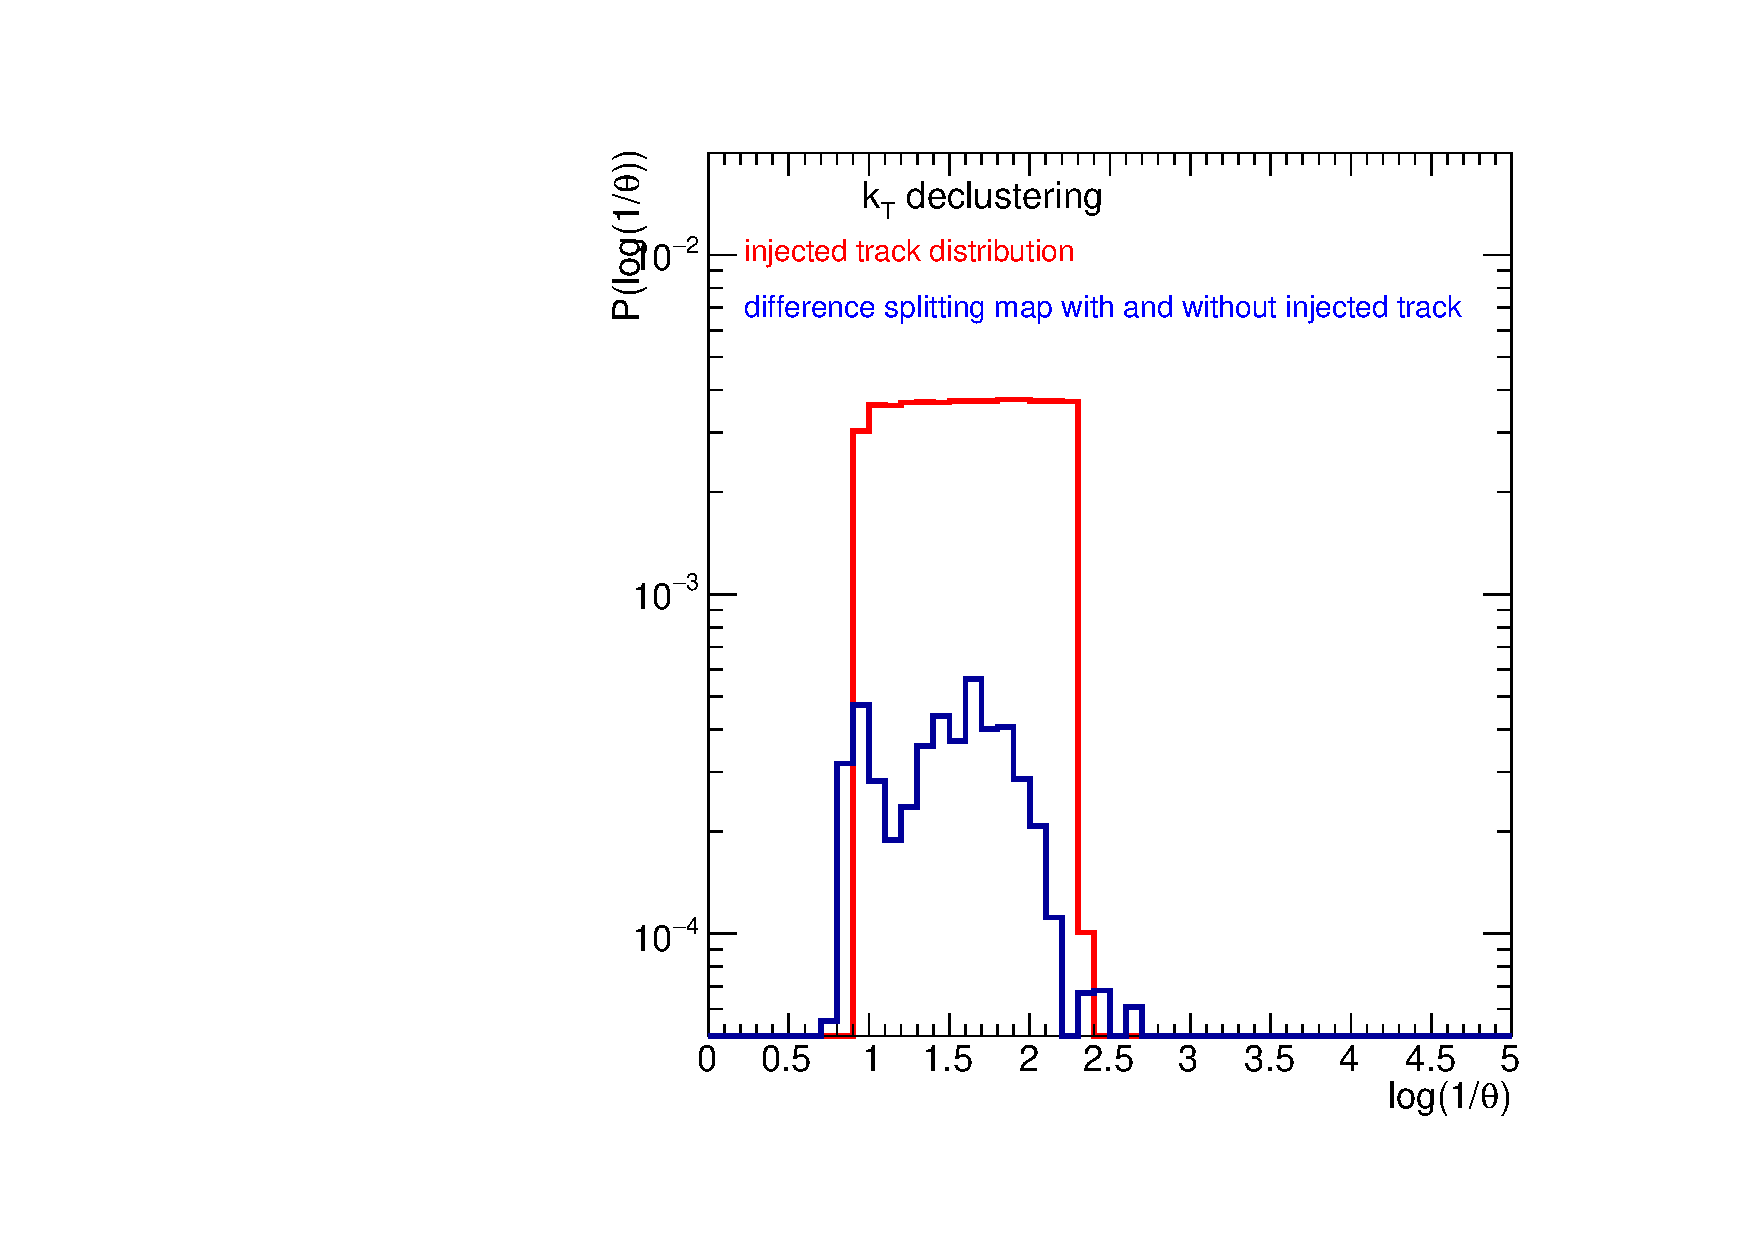
\includegraphics[width=0.3\textwidth]{figures/LundMC/projectxkt}
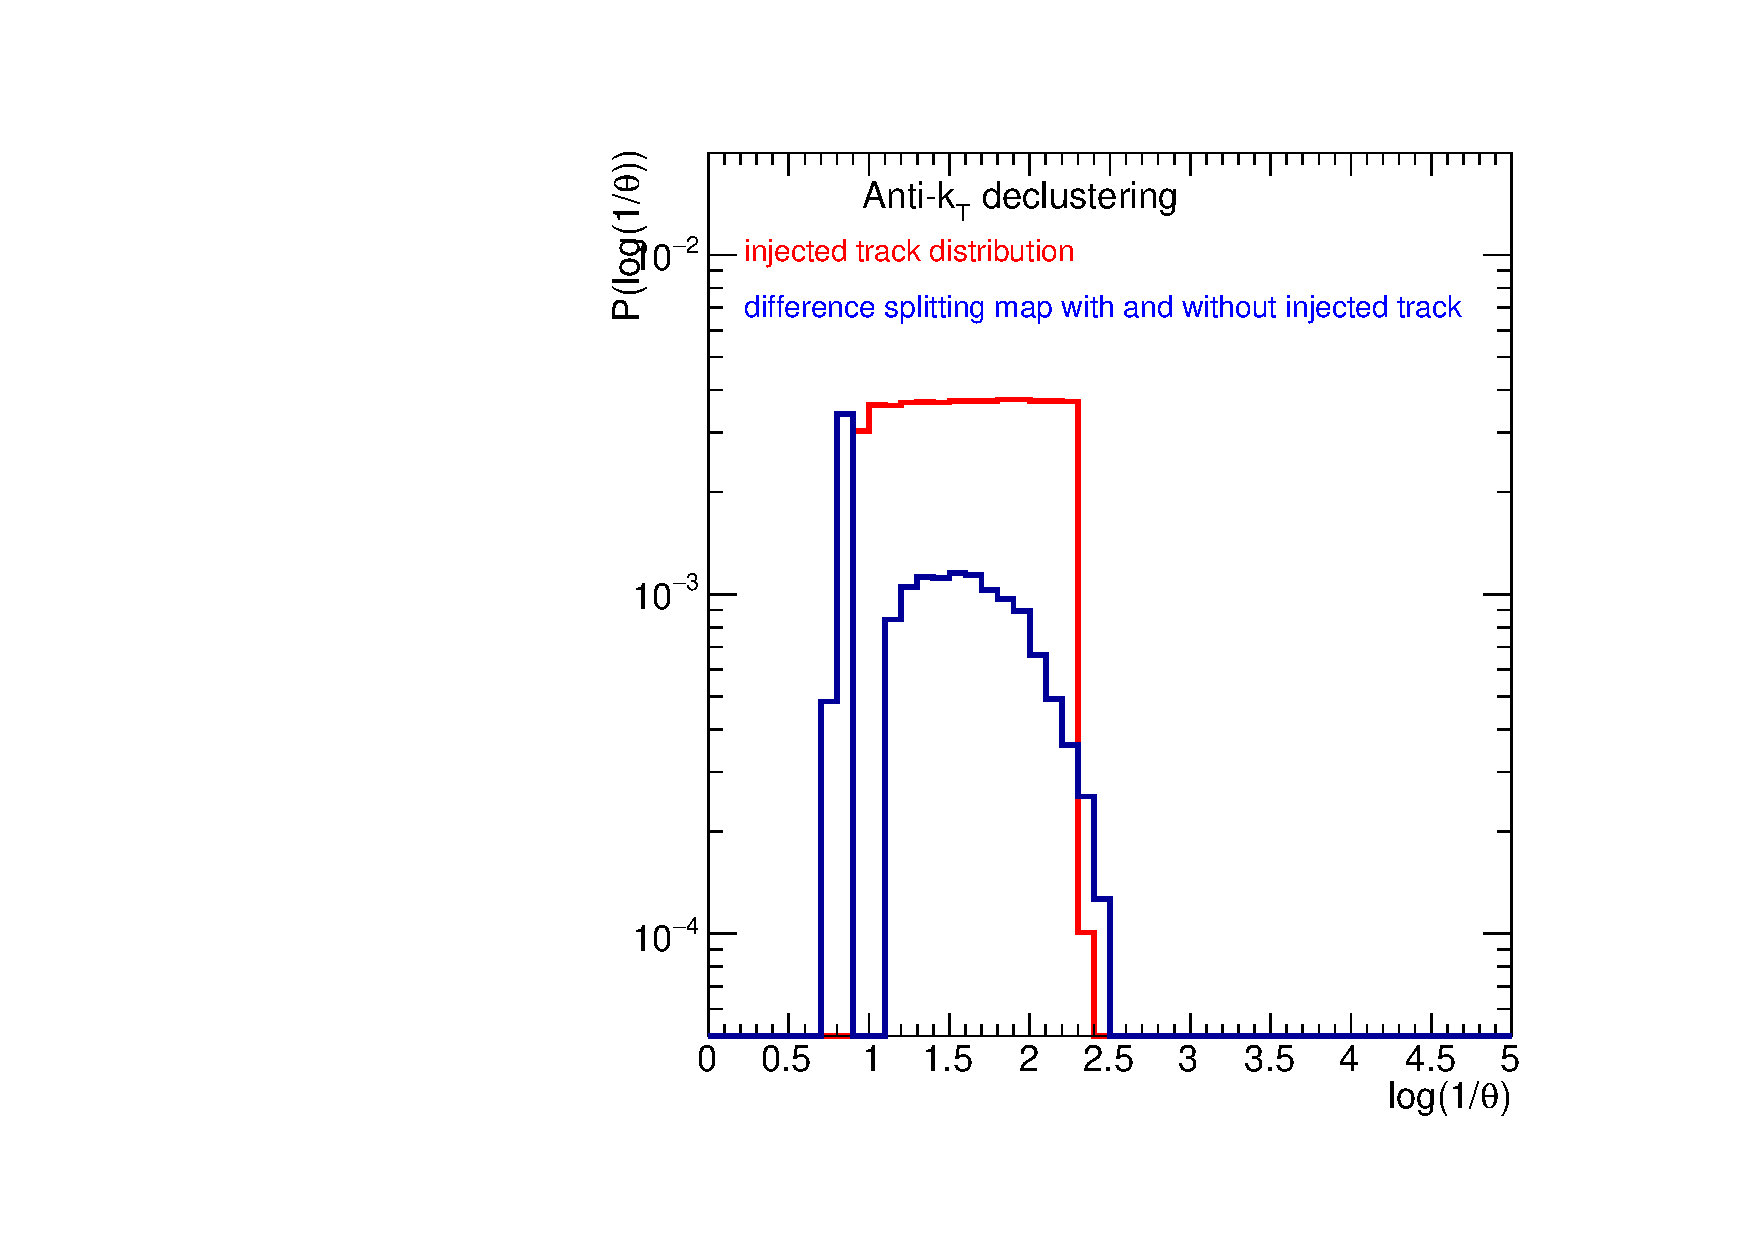
\includegraphics[width=0.3\textwidth]{figures/LundMC/projectxakt}
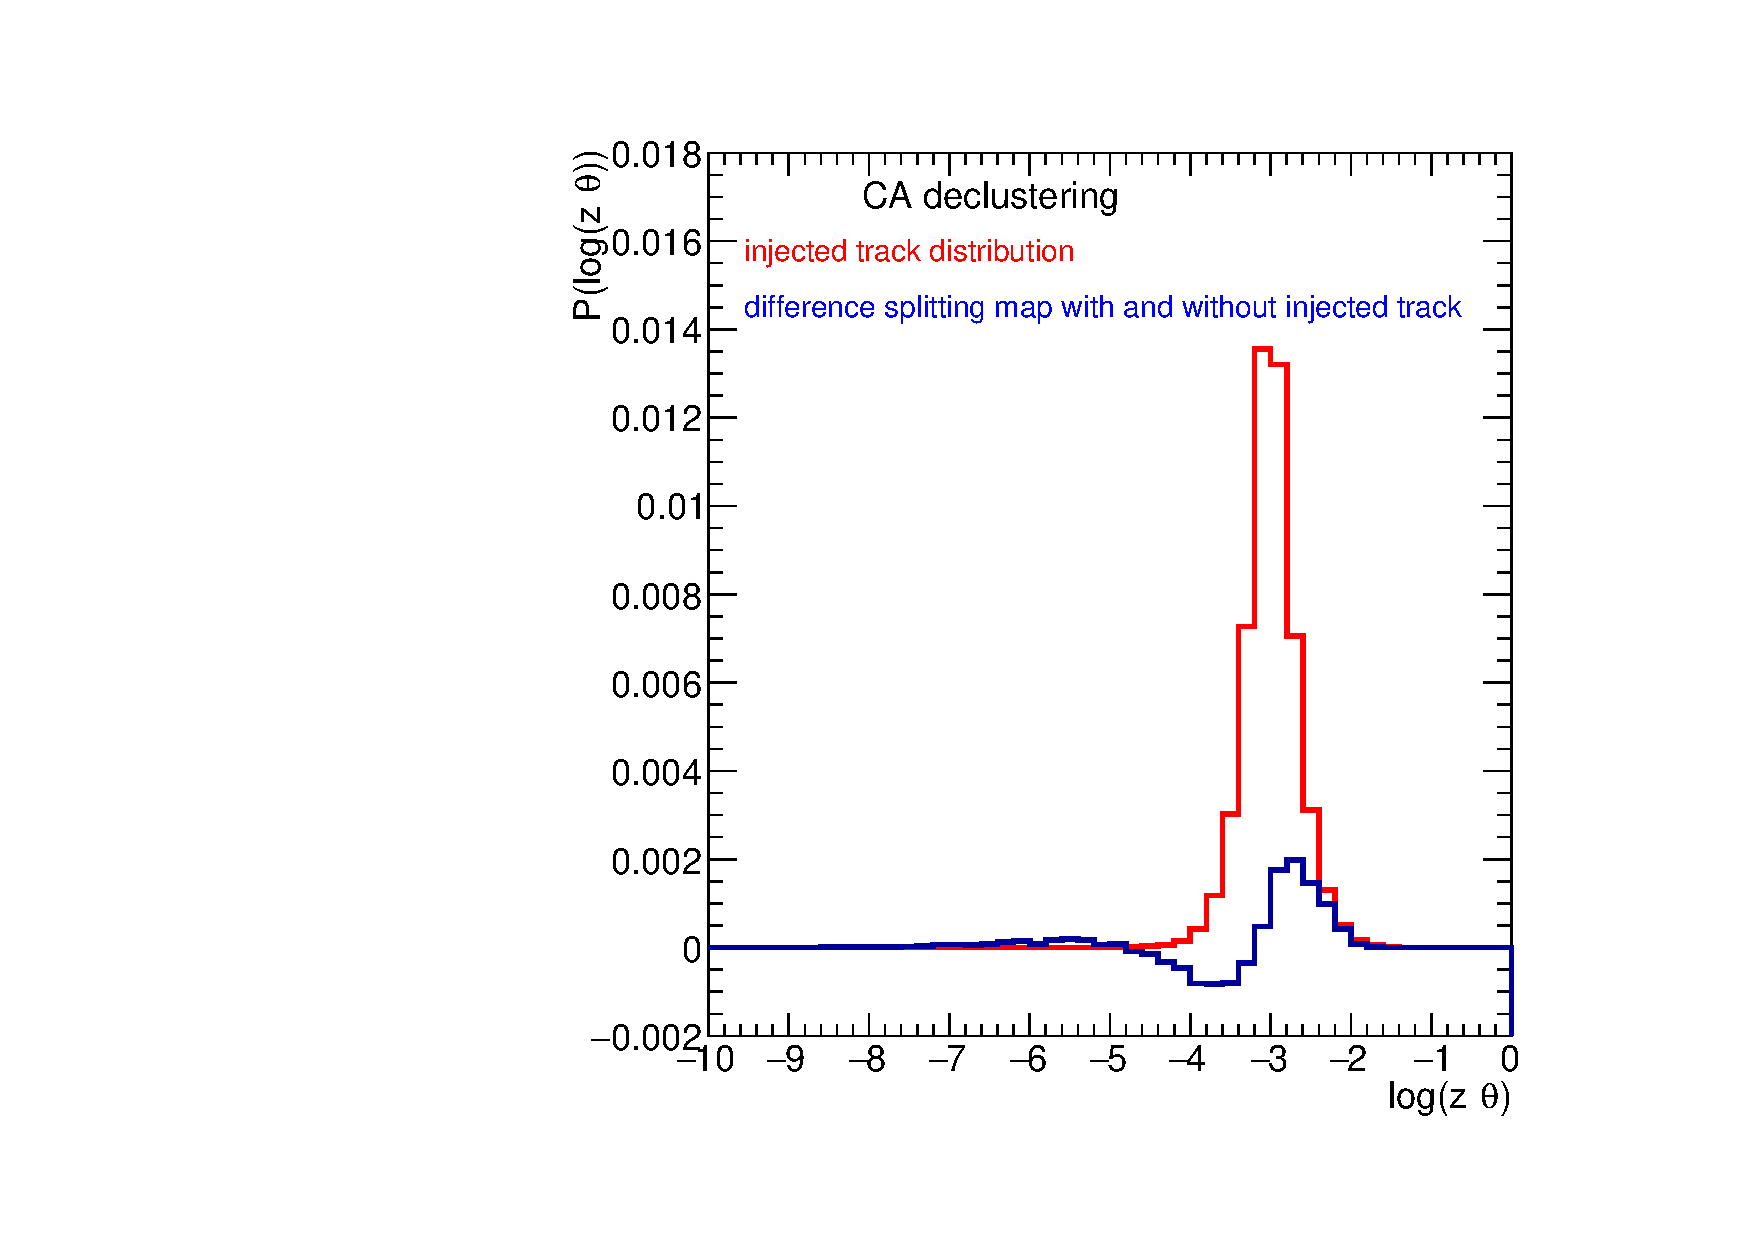
\includegraphics[width=0.3\textwidth]{figures/LundMC/projectyca}
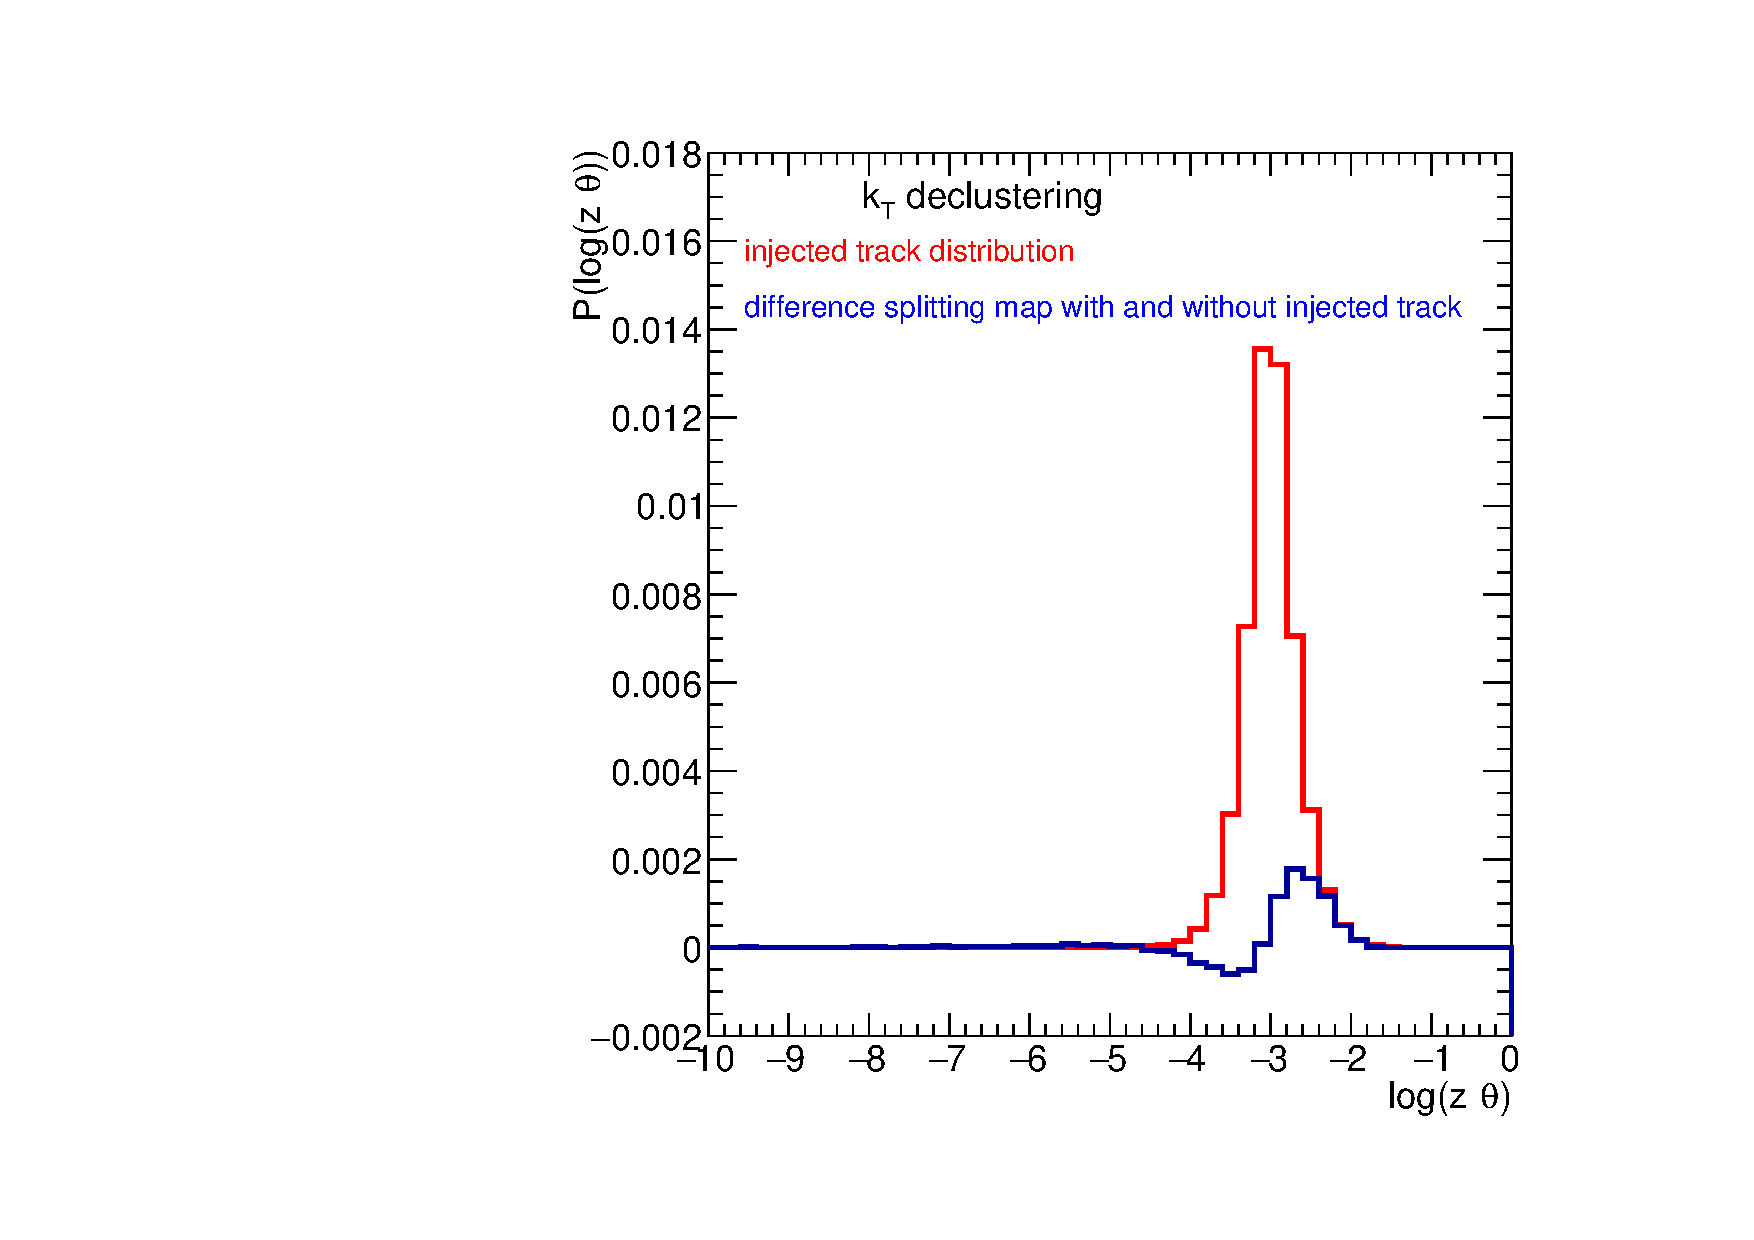
\includegraphics[width=0.3\textwidth]{figures/LundMC/projectykt}
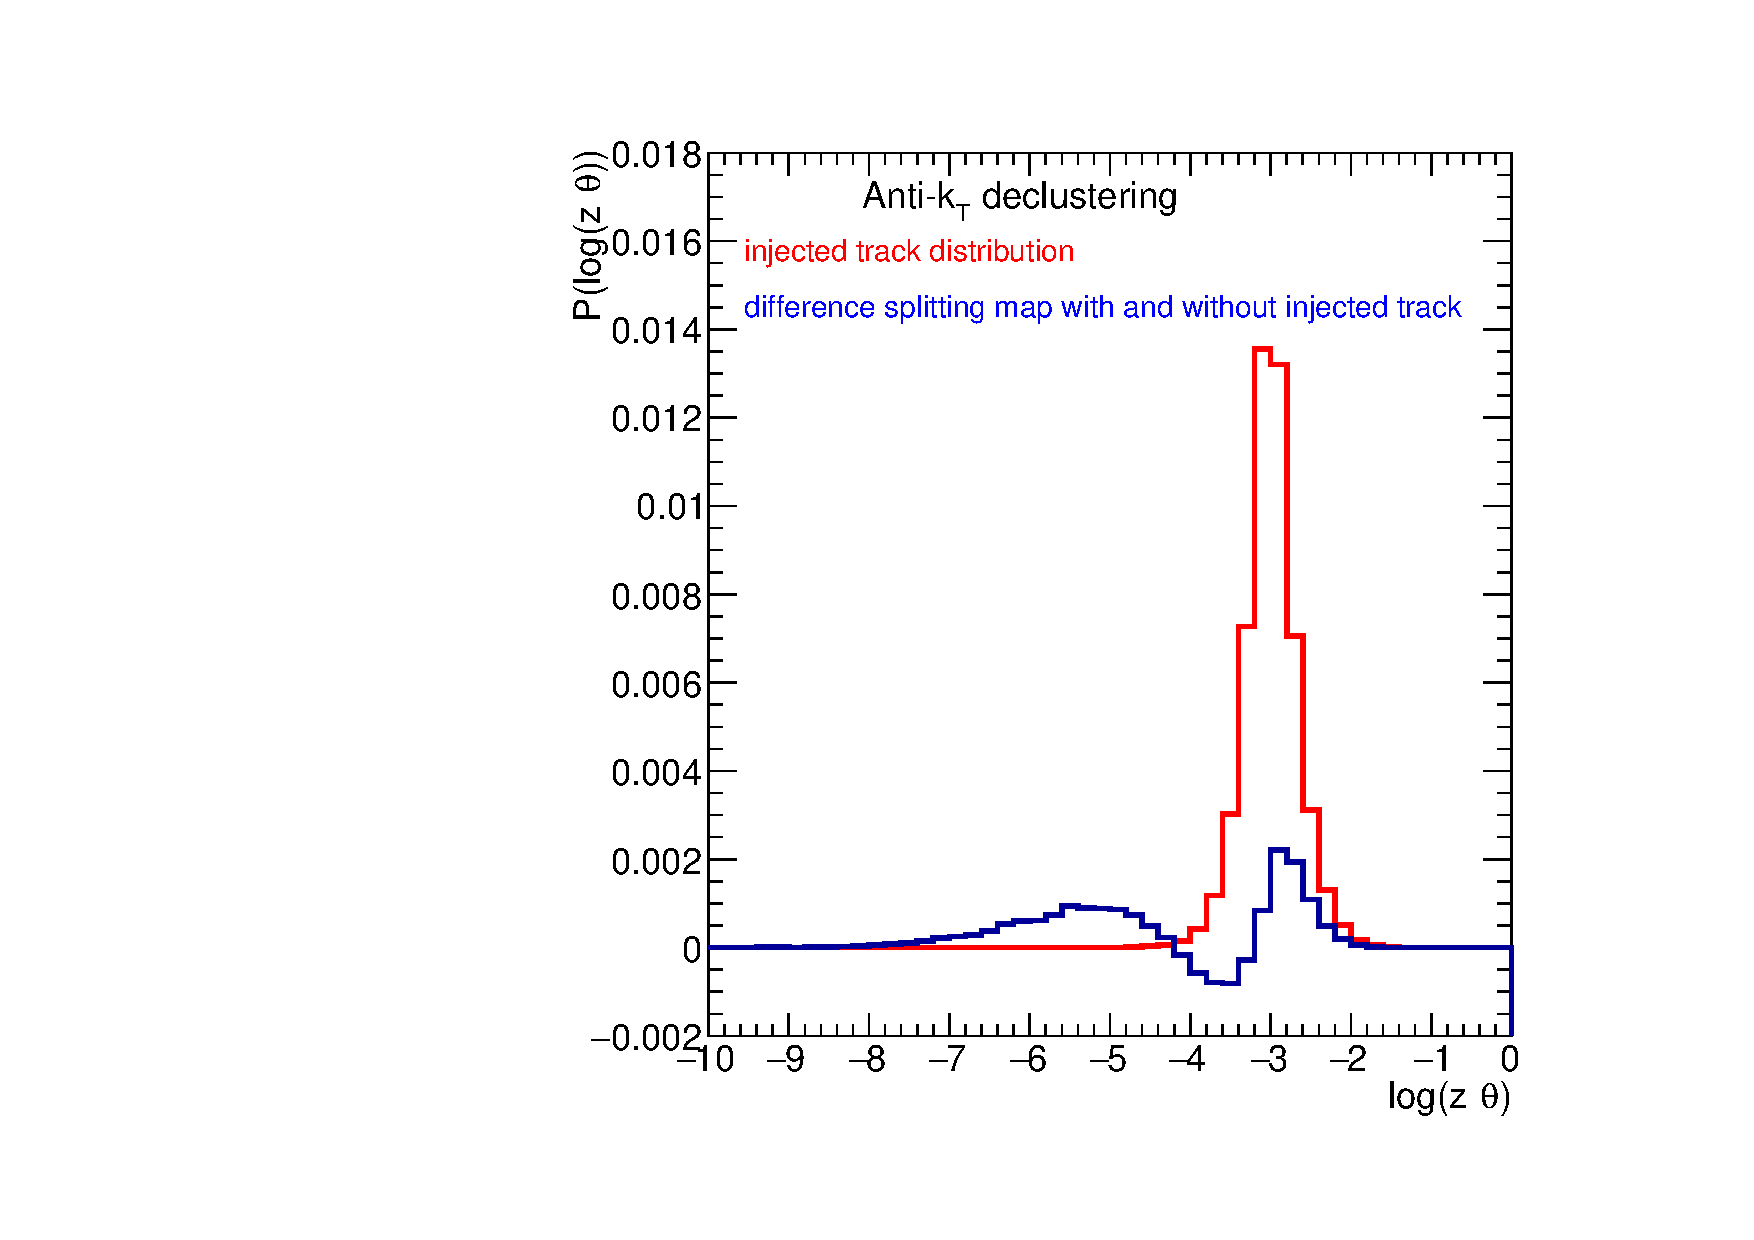
\includegraphics[width=0.3\textwidth]{figures/LundMC/projectyakt}
\caption{Projections onto x and y axes of the Lund diagram for the injected tracks and for the difference between the Lund plots of jets modified with the injected track and default jets}
\label{fig:toymodeltracks}
\end{figure}








%\subsection{Description of Monte Carlos {\color{red} Marta \& Leticia \& Liliana}}

%studies at gen-level: PYTHIA, JEWEL, Q-PYTHIA

%\subsection{Performance {\color{red} Harry \& Yen-Jie \& Phil}}
%performance plots (CS, SoftKiller discussion); jet response; subtraction methods; $\Delta R$ evolution; 

%\subsection{Some physics observables in large background {\color{red} Yen-Jie \& Yi \& Liliana \& Phil}}

%photon-jet asymmetry; $R_{AA}$; new observable $\Delta S_{12}$; substructure ($z_g$, groomed mass, $\Delta R_{12}$)
